
%----------------------------------------------------------------------------
\chapter{Preliminaries}
%----------------------------------------------------------------------------


\section{Modeling using graphs}

Structural and behavioral modeling of systems are often done using graphs. 
Graphs are useful abstraction as they are easy to understand, intuitive to use, and lots of existing algorithms can be used to process them. 
As model based approach uses models mostly of graph based formalism, in this section, graph based modeling is presented.

A directed graph consists of a set of nodes and a set of edges, where edges are a tuple of two node: its \emph{source} node and its \emph{target} node. 
Graphs can be extended to make them suitable for modeling:

\begin{itemize}
	\item by nodes having attributes with given values (e.g.\ name)
	\item by edges having labels implying their semantics
\end{itemize}


\begin{figure}[h]
	\begin{center}
		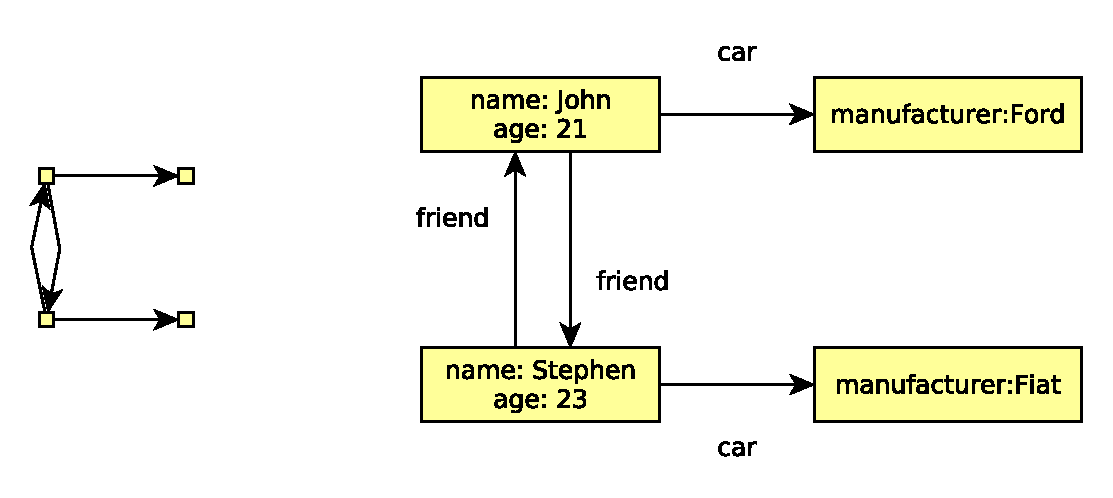
\includegraphics[width=0.75\textwidth]{figures/graphs.pdf}
		\caption{Basic graph (left), and extended (right) }
		\label{fig:graphs}
	\end{center}
\end{figure}

In case of this extended graph model we also use the term \emph{object} for nodes and \emph{reference} for edges.

With this extended graph model, there is also a need to give rules for certain types of models, which is the role of \emph{meta modeling}.
A meta model is a model, that defines how the graph model of a system is built up, i.e.\ what attributes a node has, how edges can be 



\begin{figure}[h]
	\begin{center}
		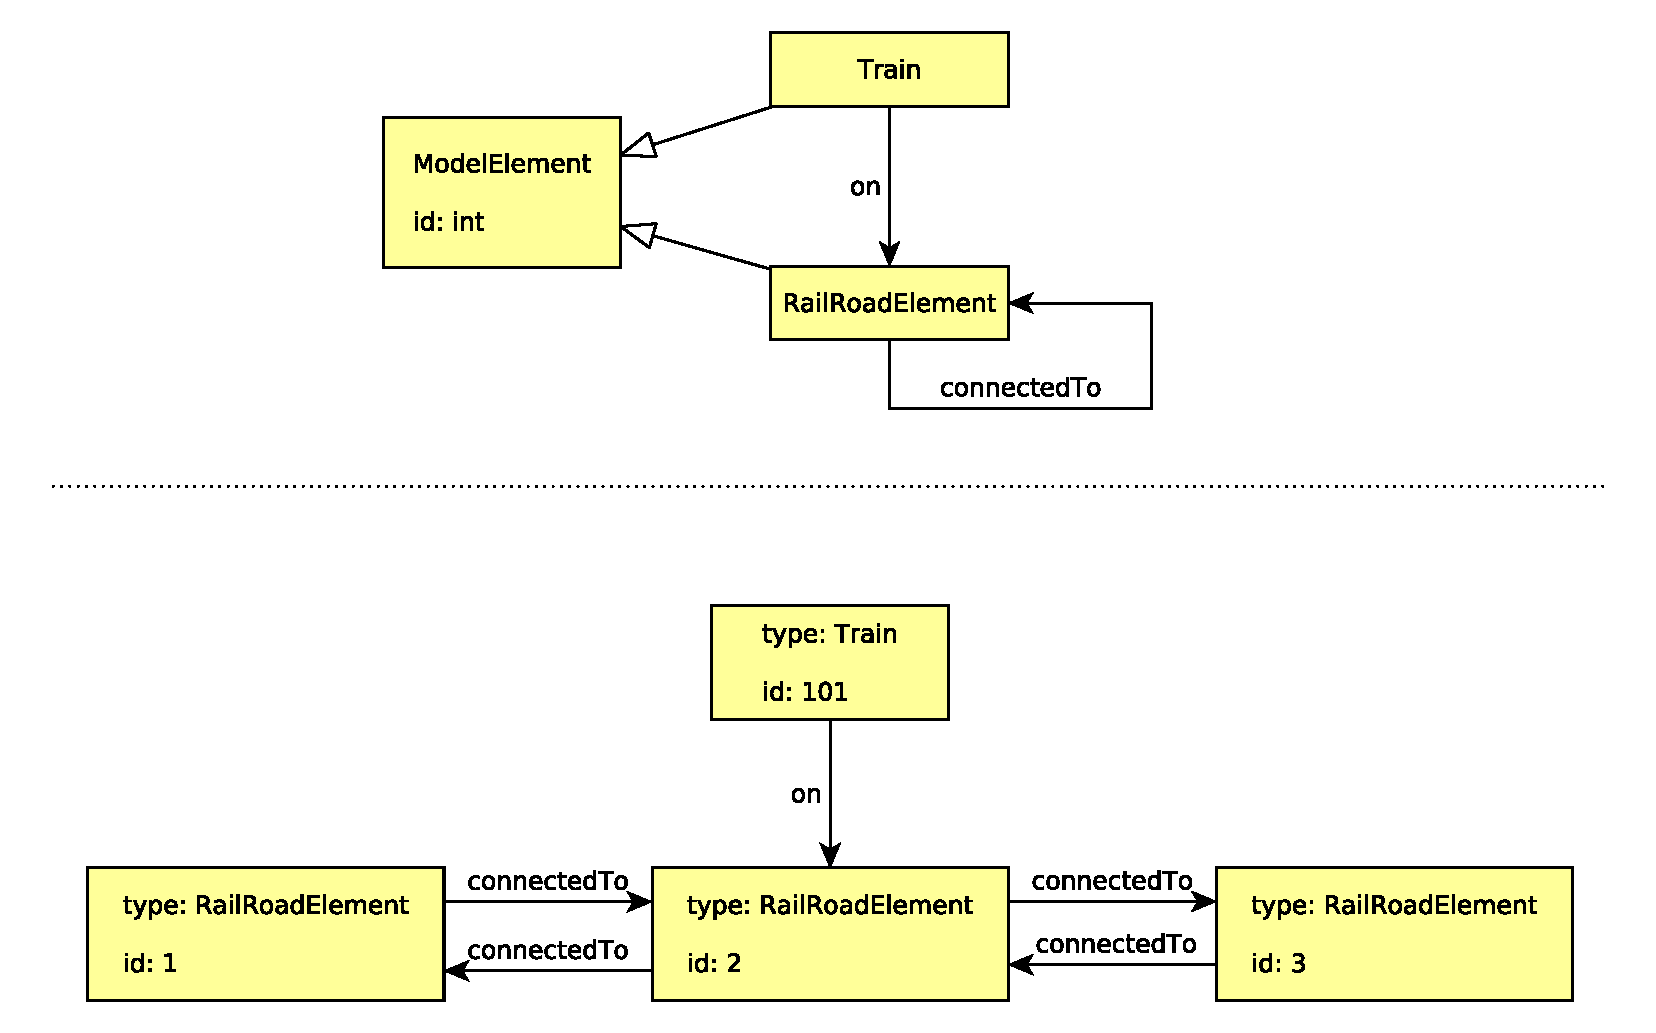
\includegraphics[width=0.75\textwidth]{figures/metamodel.pdf}
		\caption{ Example of a metamodel and an intance model }
		\label{fig:metamodel}
	\end{center}
\end{figure}


\section{Domain and runtime modeling}

In this framework, we use structural modeling to model the current state of the system. 
The state and the operating context of the system is captured in a model called the \emph{live model}.
It is updated with sensor data and information from other sources, so the model represents the physical system's latest state. 
This model can be used to infer problems in the state of the system, so it can be used for runtime verification.


\todo{Értelmes ábrát ide}
\begin{figure}[h]
	\begin{center}
		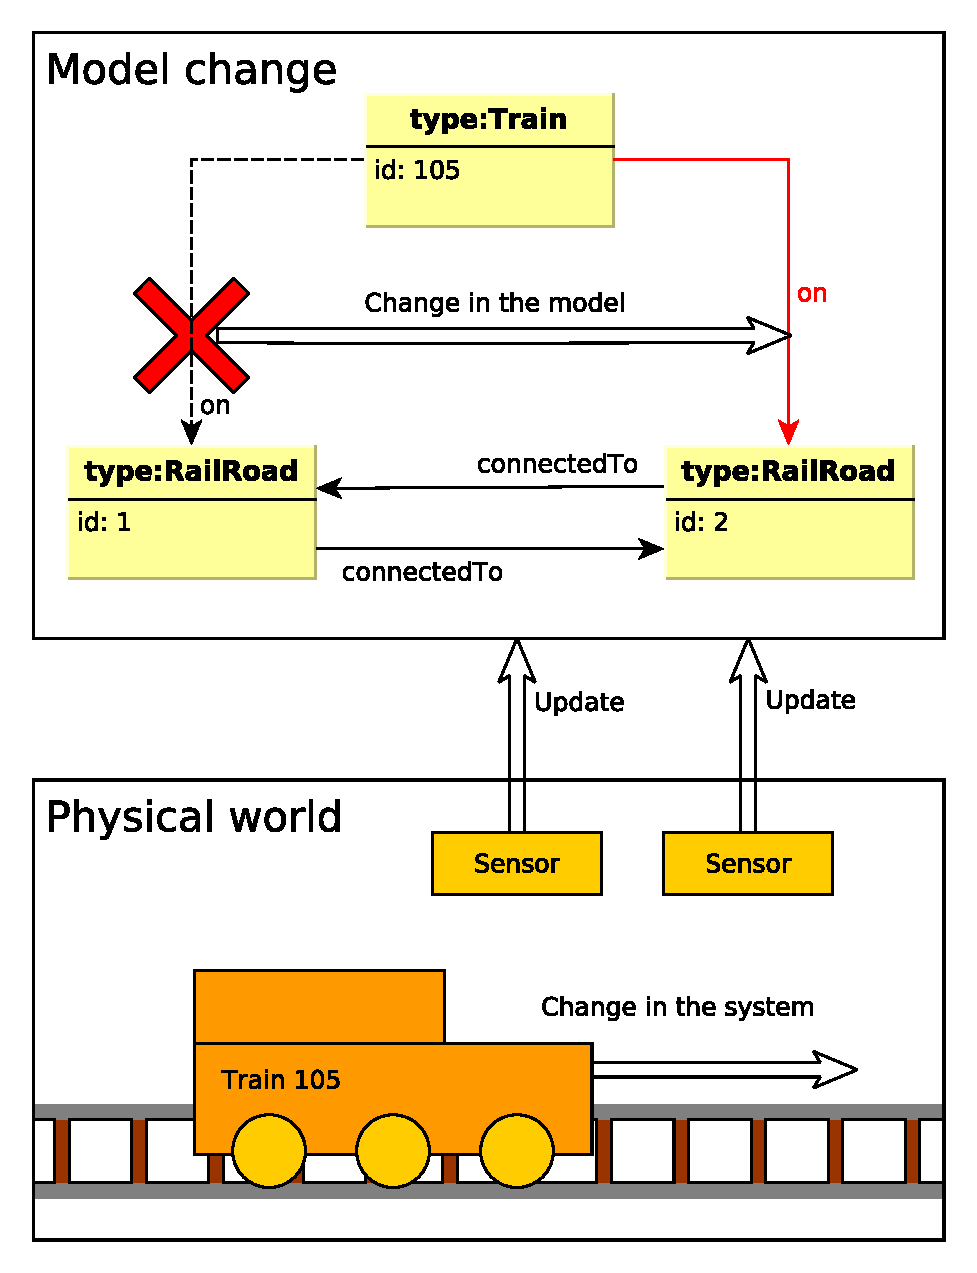
\includegraphics[width=0.75\textwidth]{figures/live-models.pdf}
		\caption{Live model updating}
		\label{fig:live-models}
	\end{center}
\end{figure}

\section{Graph pattern matching concepts}
\label{section:gpmc}

As runtime analysis of the system is based on the runtime model, we needs to identify problems in the graph model. 
Graph pattern matching offers a solution for this problem. 
The goal of graph pattern matching is to find all the subgraphs of a graph meeting a certain criteria, defined by a \emph{graph pattern}.

A \emph{graph pattern} is given by a \emph{restricted} first-order logical expression, where variables refer to vertices of the graph or data values (string, numeric, enumeral).
Free(not quantified) variables are called \emph{parameters}.  
A \emph{pattern match} is a variable binding, where variables are assigned to graph nodes and data values in a way, that satisfies the expression.
A pattern's \emph{matchset} on a graph is the set of all the possible pattern match (ie. the truth set of the graph pattern if we view it as a predicate on the parameters).
A \emph{graph query} is a program or execution plan capable of calculating the matchset of a graph pattern on a given graph. 
Planning the most efficient graph query is crucial, because the performance of the verification depends on it.

Graph patterns are built up from basic constraints. 
A constraint is a predicate on a tuple of variables. 
These constraints are: 

\begin{itemize}
	\item Type constraint -- Satisfied, when the variable's value is a vertex of a given type
	\item Reference -- Satisfied, when an edge with a given label exists from the first variables value to the second variables value
	\item Equality -- two variable's value is the same
	\item Inequality -- two variable's values are different
	\item Pattern match -- a tuple of variable values are a match of another pattern
	\item Negative application condition (NAC) -- a tuple of variable values are \emph{not} a match of another pattern
\end{itemize}


We built up the expression defining the graph pattern the following way. 
An expression is a logical conjunction of subexpressions called pattern bodies ($Pattern = B_1 \vee B_2 \vee \dots$). 
A \emph{pattern body} is an existentially quantified expression, quantified over a disjunction of constraints ($\exists{} v_1, v_2, \dots : C_1 \wedge{} C_2 \wedge \dots$).

Viatra Query Language syntax conform with this structure as this restriction leads to more easily understandable graph queries.
This restriction also helps our expressions to become evaluable using local search.

We can also use a visual representation (see Fig. \ref{fig:pattern-visual}) to illustrate a graph pattern, altough textural languages (see VQL) is used in the framework.

\begin{figure}[h]
	\begin{center}
		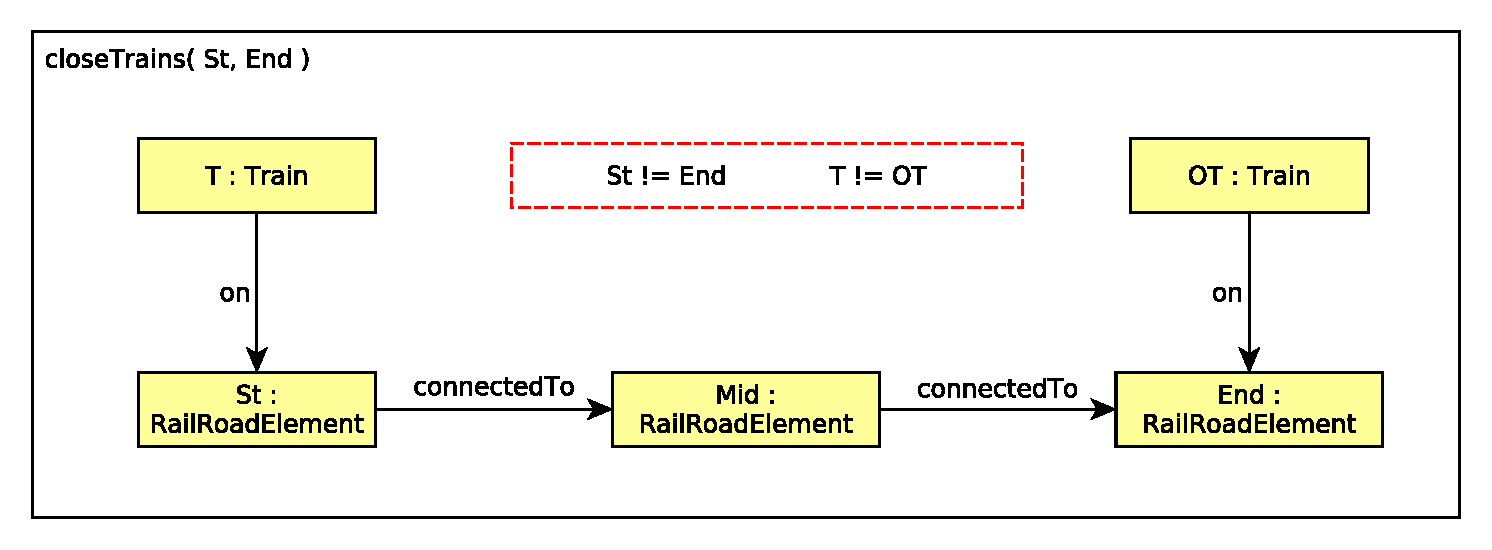
\includegraphics[width=\textwidth]{figures/closeTrains-pattern.pdf}
		\caption{Non-formal visual representation of a graph pattern}
		\label{fig:pattern-visual}
	\end{center}
\end{figure}


\section{Local search}

Local search is a method for solving problems involving a search space. 
Local search starts from a candidate solution for a problem, then searches by applying local changes: moving to neighboring locations until solutions are found.

Local search can also be used to provide a matchset for a graph pattern in a graph.
It is also a memory-efficient alternative for rete algorithm in \viatra{}~\cite{bur-marton-msc}.

One of the possibility (also used in ~\cite{bur-marton-msc} and our framework) is the following :
Assume, that a graph pattern is given as stated before in section~\ref{section:gpmc}.
Then it is a conjunction of expressions (bodies) that existentially quantifies the variables, then checks if the constraints are met.

\begin{equation}
\begin{array}{@{}r@{\,}l@{\,}l@{}}
foo &= bar &+ baz\\
&= bar &+ quux
\end{array}
\end{equation}


\begin{equation}
\begin{array}{@{}r@{}l@{}l@{}l@{}l@{}l@{}}
Pattern(p1, p2, \dots) = \;
& \exists{x_1} & \exists{x_2}... \: & 
(Constr_{11}(\bar{p},\bar{x} ) & \, \wedge \, Constr_{12}(\bar{p},\bar{x} ) & \, \wedge \, \dots{}) \: \vee \\

& \exists{y_1} & \exists{y_2}... \: & 
(Constr_{21}(\bar{p},\bar{y} ) & \, \wedge \, Constr_{22}(\bar{p},\bar{y} ) & \, \wedge \, \dots{}) \: \vee \\
& \dots{}
\end{array}
\end{equation}

We can find the truth set of this expression, by finding the truth sets of all the bodies as distinct predicates on the parameters, and taking their union.
Our problem now is the following: find all the variable bindings, which satisfies the constraints of the body.

\todo{ez itt finomítható}

The search space consists of all the possible variable bindings (leaving a variable unbind is also a possibility). 
We start from all variable being unbound. 
We go through the constraints and with each constraint, we do one of the following:
\begin{itemize}
	\item Check operation: If all the variables referred by the constraint are bound, then we check if they satisfy the constraint. If yes, we follow the algorithm, if not we backtrack.
	\item Extend operation: If a variable is unbound then we iterate through all the possible values that satisfies the constraint, and for each value we bind it to the variable and follow the algorithm. After all the possible values are done, we backtrack.
\end{itemize}

This structure leads to a search tree.
It can be easily proved, that at the ith of the tree, the first x constraint is satisfied, as a child node not modifies already bound variables.
This means, that after the last constraint, the variable binding satisfies all the constraints, so it can be projected to the variables to find a solution.
It can also be proved, that all of the variable bindings satisfying the constraints can be found: 
Consider this variable bindings, and call this the goal binding, and start the algorithm: each extend operation can bind the unbound variables as in the goal binding, and each check operation 

We use depth first search, because it uses less memory, and it can be easily used to synthesize code, as the layers are well defined. This way search can be easily implemented using nested for loops.


\section{Distributed platform}

% adatok diszjunkt halmazokra bontva különböző csomópontra
% az algoritmusok is elosztottak, nem lesz összegyűjtve az infó, úgy van kiértékelve, hogy nincs aki mindent látna a rendszerből

As cyber-physical systems are distributed we must deal with the sensor data coming from different sensors at different computation units of the system. 
Sending the sensor data to one computation unit and evaluate on that can cause different problems: 
Sensor data can be too huge to be able to be sent over network, the central node can be a SPOF~(Single Point of Failure), etc. 

In the presented framework the live model is distributed on the different computation units and the graph pattern matching algorithm itself runs in a distributed way. 
This eliminates the problem of central computers, but introduces complexity, that we must handle.
One of the problems is distributed model handling, and the other is how to execute queries efficiently on a distributed platform.

\subsection{Distributed graph modeling}

In this thesis, the phrase \emph{computing module} is used to denote a physical or virtual execution component of the cps that is capable of storing a part of the graph model and updates it to fit the current state the physical world, eg.\ an embedded system or a virtual machine.

Distributed graph models can be architected in various ways. 
In our framework each node in the graph is allocated to a computing element. 
On that computing element, that node is called a \emph{local node}. 
In the context of other computing modules it is called a \emph{remote node}. 
Edges are stored in the computing module of their source node; 
If their destination node is not a local node on that node, a \emph{proxy node} is used to substitute the remote node.


\begin{figure}[h]
	\begin{center}
		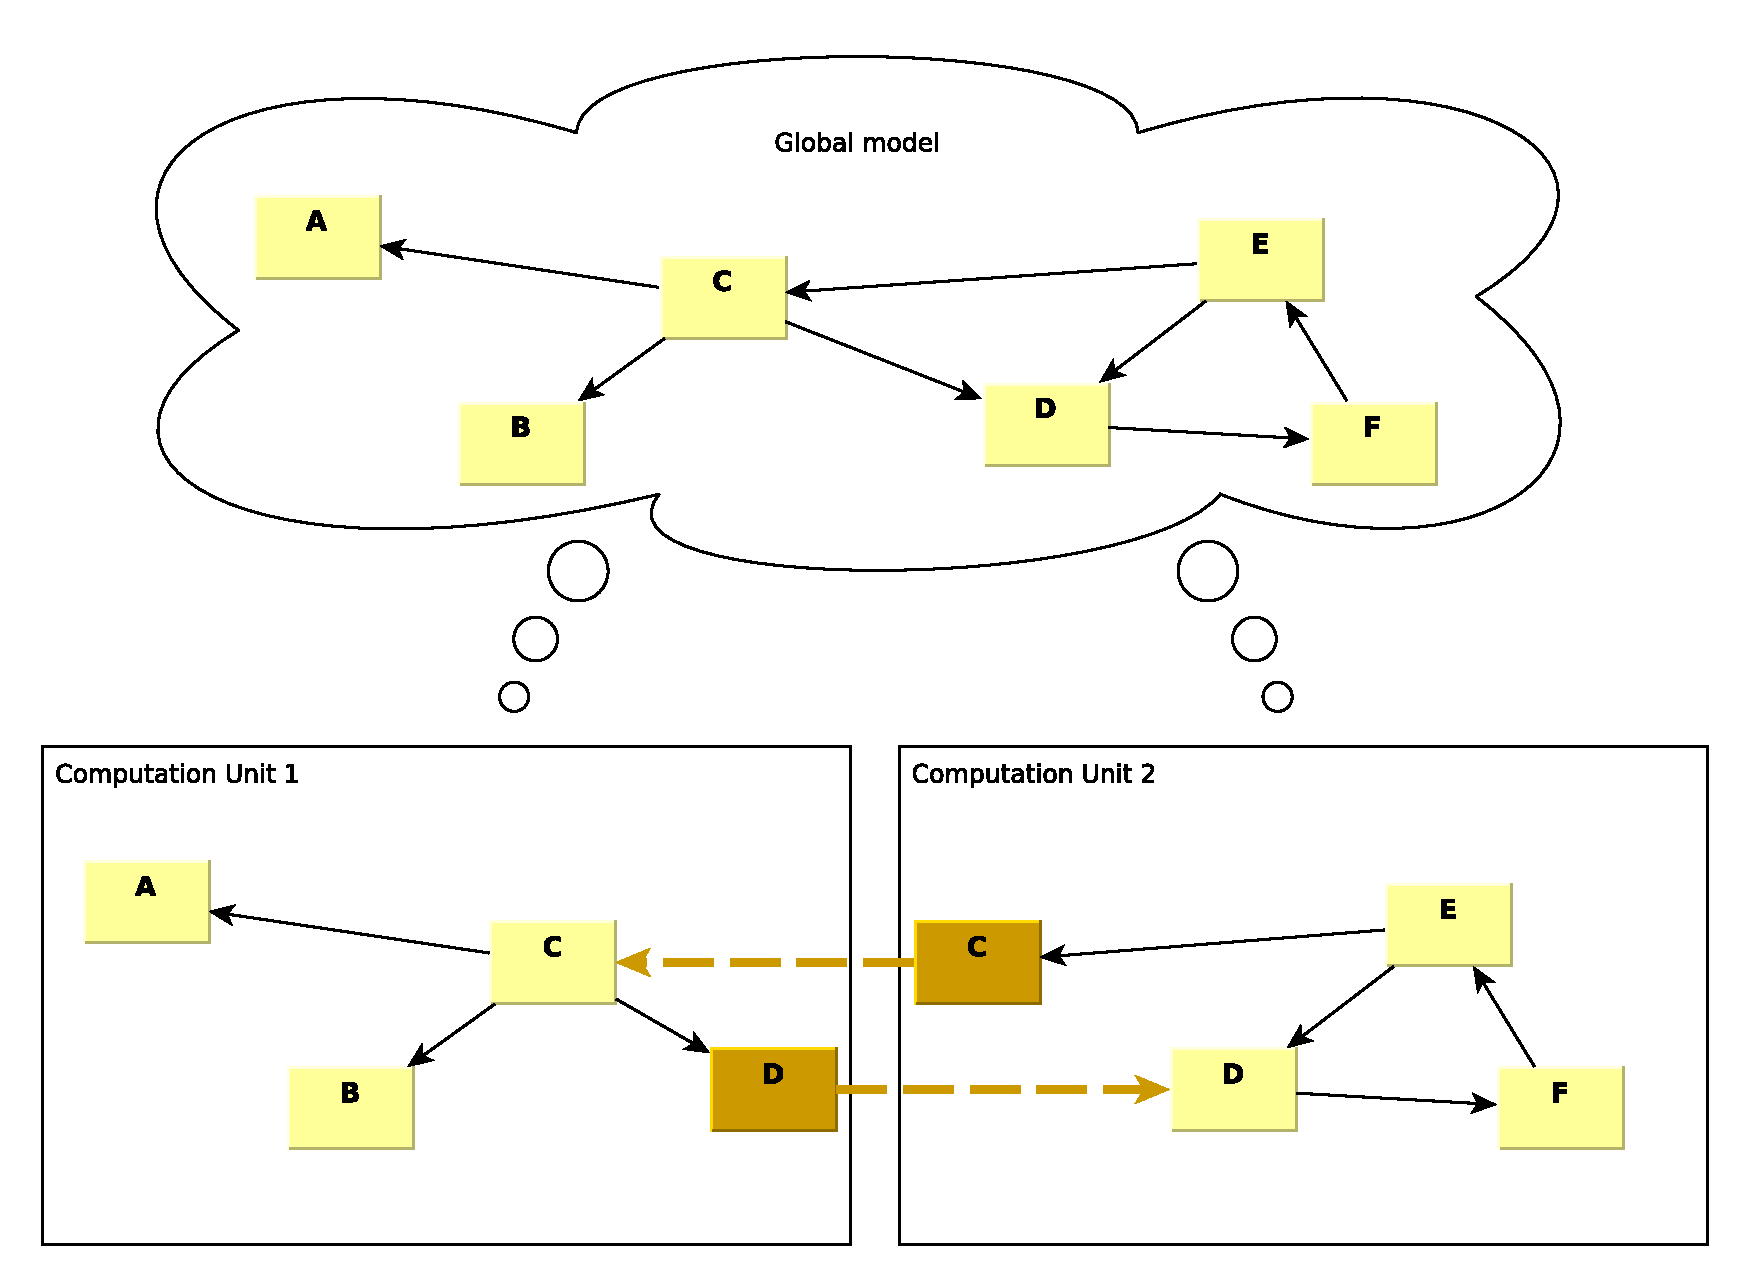
\includegraphics[width=\textwidth]{figures/distributed-model-handling.pdf}
		\caption{Handling distributed models and cross-references}
		\label{fig:distributed-model-handling}
	\end{center}
\end{figure}



\subsection{Distributed query execution}

Distributed query execution is used in the framework to provide matches to graph patterns. 
A distributed local search planner shall consider distributed execution to improve its output plan execution performance.







